\section{ラグランジュ補間多項式とその評価} % 一章
\label{sec:lagrange_interpolation}
  本章では，まずラグランジュ補間多項式の基礎理論と本研究で導出された多項式の評価方法についてについて述べる．
  
  \subsection{ラグランジュ補間多項式の導出と一意性}
  \label{subsec:lagrange_derivation}
    $n$次補間多項式とは，与えられた$n+1$個の標本点をすべて通る$n$次以下の多項式である．
    異なる $n+1$ 個の標本点 $(x_0, y_0), \dots, (x_n, y_n)$ が与えられたとき，これらすべての点を通る $n$ 次以下の多項式 $p_n(x)$ は一意に存在する．
    求める多項式を \[p_n(x) = c_0 + c_1 x + \dots + c_n x^n\] とおくと,
    この多項式の補間条件 \[p_n(x_i) = y_i \quad (i=0,\dots,n)\] は，以下の係数 $c_j$ に関する連立一次方程式に帰着される．

    \begin{equation}
    \left(
    \begin{array}{cccc}
    1 & x_0 & \cdots & x_0^n \\
    1 & x_1 & \cdots & x_1^n \\
    \vdots & \vdots & \ddots & \vdots \\
    1 & x_n & \cdots & x_n^n
    \end{array}
    \right) 
    \left(
    \begin{array}{c}
    c_0 \\
    c_1 \\
    \vdots \\
    c_n
    \end{array}
    \right)
    =
    \left(
    \begin{array}{c}
    y_0 \\
    y_1 \\
    \vdots \\
    y_n
    \end{array}
    \right).
    \label{eq:matrix_interp}
    \end{equation}

    この係数行列はファンデルモンド行列と呼ばれ，標本点が異なるならば行列式は非ゼロとなり係数が一意に定まること知られている\cite{suchikaiseki-nyumon}．

  \label{subsec:error_function}
  \subsection{誤差関数}
    誤差関数とは多項式と元の関数 $f(x)$ との差を表す関数である．
    具体的には，関数 $f(x)$ とその補間多項式 $p_n(x)$ に対して，誤差関数 $e(x)$ は次のように定義される．
    \begin{equation}
      e(x) = f(x) - p_n(x).
    \end{equation}
    この誤差関数は，補間多項式が元の関数をどれだけ正確に近似しているかを評価するために用いられる．
    補間多項式の次数 $n$ を増加させることで，一般に誤差関数の絶対値は小さくなる傾向がある．
\label{subsec:polynomial_methods}
  
  \subsection{多項式近似の手法：テイラー展開と補間多項式}
    多項式を用いた関数近似には，大きく分けて二つの手法が存在する．
    \begin{enumerate}
      \item \textbf{テイラー展開}：特定の点での微分情報を用いて，その近傍で高精度な近似を得る方法
      \item \textbf{補間多項式}：複数の点での関数値を通る多項式を求める方法
    \end{enumerate}
    
    本章では，特に補間多項式のアプローチに注目し，その成功例と失敗例を示すことで，
    良い近似を得るための標本点選択の重要性を学ぶ．
\label{subsec:taylor_expansion}
  
  \subsection{テイラー展開による近似}
    まず，テイラー展開による多項式近似の例を示す．
    $f(x) = \sin(x)$ を $x = 0$ の周辺で展開すると，
    \[T_n(x) = x - \frac{x^3}{3!} + \frac{x^5}{5!} - \cdots + \frac{(-1)^n x^{2n+1}}{(2n+1)!} .\]
    
    テイラー展開は展開中心点 $x=0$ 付近では極めて高精度であり，
    $[-\pi/2, \pi/2]$ の範囲でも非常に良好な近似が得られる．
    
    \clearpage
    % =========================================================
    % テイラー展開による近似
    % Goプログラム (sin_taylor_unified.go) が生成した
    % テイラー多項式の可視化ファイルを読み込む
    % =========================================================
    % sin関数のテイラー展開による近似比較図

\begin{figure}[H]
  \centering
  \caption{$f(x) = \sin(x)$のテイラー展開（3次多項式）}
  \label{fig:sin-taylor-first}
  \vspace{5pt}
  \begin{minipage}[b]{0.48\linewidth}
    \centering
    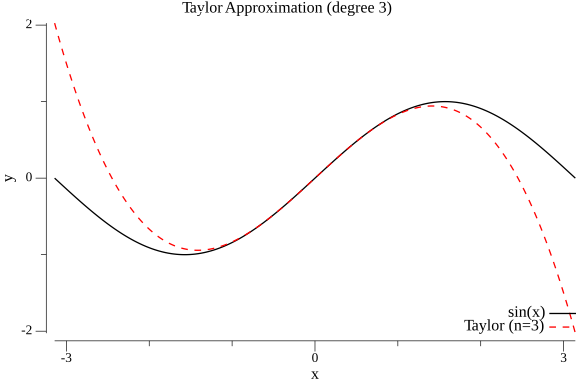
\includegraphics[width=1.0\linewidth]{material/sin/taylor/sin_taylor_n01.png}
  \end{minipage}
  \hfill
  \begin{minipage}[b]{0.48\linewidth}
    \centering
    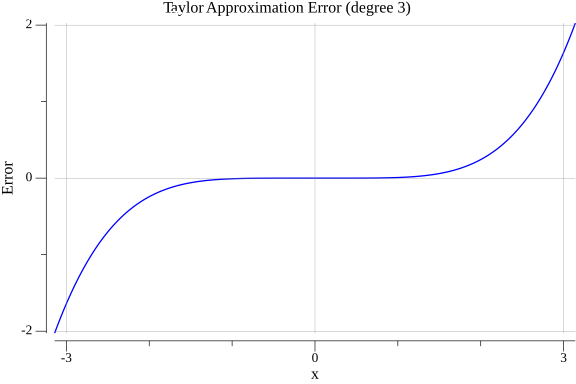
\includegraphics[width=1.0\linewidth]{material/sin/taylor/sin_taylor_err_n01.png}
  \end{minipage}
\end{figure}

\begin{figure}[H]
  \centering
  \caption{$f(x) = \sin(x)$のテイラー展開（11次多項式）}
  \label{fig:sin-taylor-2}
  \vspace{5pt}
  \begin{minipage}[b]{0.48\linewidth}
    \centering
    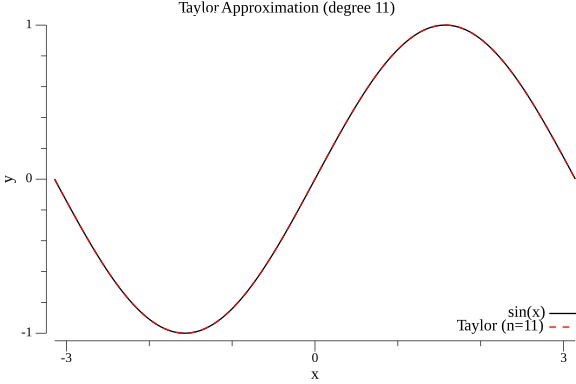
\includegraphics[width=1.0\linewidth]{material/sin/taylor/sin_taylor_n05.png}
  \end{minipage}
  \hfill
  \begin{minipage}[b]{0.48\linewidth}
    \centering
    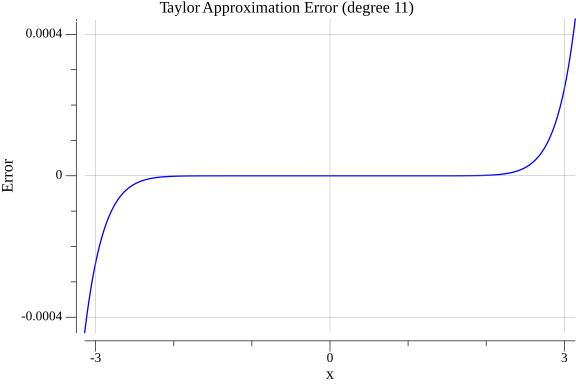
\includegraphics[width=1.0\linewidth]{material/sin/taylor/sin_taylor_err_n05.png}
  \end{minipage}
\end{figure}

\begin{figure}[H]
  \centering
  \caption{$f(x) = \sin(x)$のテイラー展開（23次多項式）}
  \label{fig:sin-taylor-last}
  \vspace{5pt}
  \begin{minipage}[b]{0.48\linewidth}
    \centering
    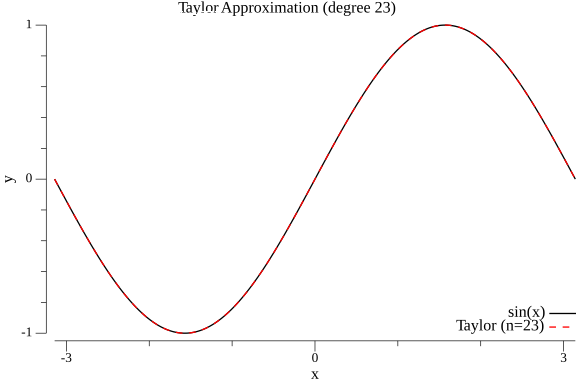
\includegraphics[width=1.0\linewidth]{material/sin/taylor/sin_taylor_n11.png}
  \end{minipage}
  \hfill
  \begin{minipage}[b]{0.48\linewidth}
    \centering
    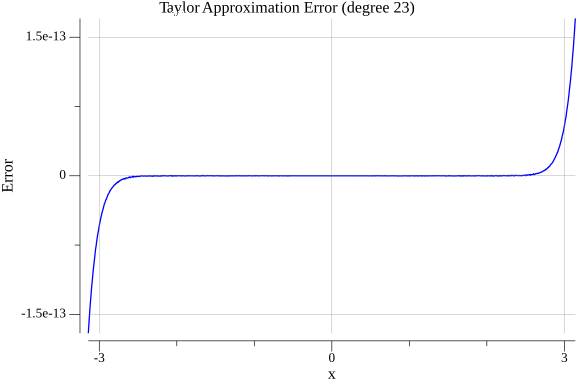
\includegraphics[width=1.0\linewidth]{material/sin/taylor/sin_taylor_err_n11.png}
  \end{minipage}
\end{figure}



    テイラー展開は展開中心点付近では優れた近似性を持つが，
    中心点から遠く離れた領域では精度が低下する傾向がある．
    

  \subsection{ラグランジュ補間多項式による近似：成功例}
    一方，ラグランジュ補間多項式 $p_n(x)$ は，$n+1$個の標本点を補完する多項式を構成する方法である．
    補間多項式の精度は，標本点の選択方法に大きく依存する．
    
    成功例として，$f(x) = \sin(x)$ を $[-\frac{\pi}{2}, \frac{\pi}{2}]$ で補間する場合を考える．
    sin関数は等間隔点による補間でもある程度の精度を得ることができる．
    
    \clearpage
    % =========================================================
    % sin関数による成功例
    % Goプログラム (sin_unified.go) が生成した
    % 等間隔補間の可視化ファイルを読み込む
    % =========================================================
    % sin関数の等間隔補間による比較図

\begin{figure}[H]
  \centering
  \caption{$f(x) = \sin(x)$の等間隔補間（$n=1$次多項式）}
  \label{fig:sin-interp-first}
  \vspace{5pt}
  \begin{minipage}[b]{0.48\linewidth}
    \centering
    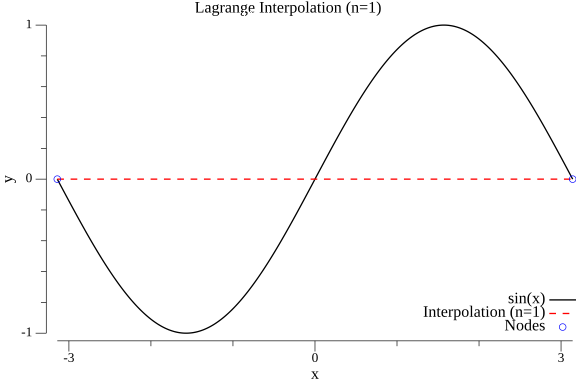
\includegraphics[width=1.0\linewidth]{material/sin/interp/sin_interp_n01.png}
  \end{minipage}
  \hfill
  \begin{minipage}[b]{0.48\linewidth}
    \centering
    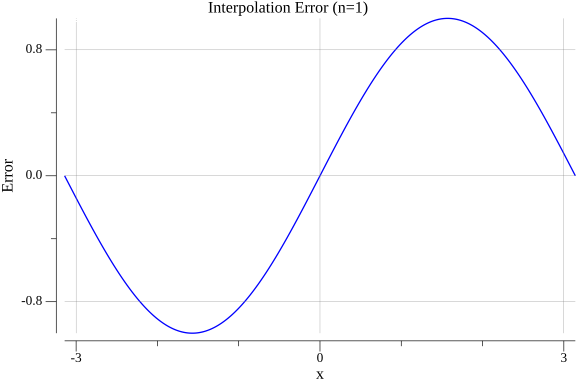
\includegraphics[width=1.0\linewidth]{material/sin/interp/sin_interp_err_n01.png}
  \end{minipage}
\end{figure}

\begin{figure}[H]
  \centering
  \caption{$f(x) = \sin(x)$の等間隔補間（$n=5$次多項式）}
  \label{fig:sin-interp-2}
  \vspace{5pt}
  \begin{minipage}[b]{0.48\linewidth}
    \centering
    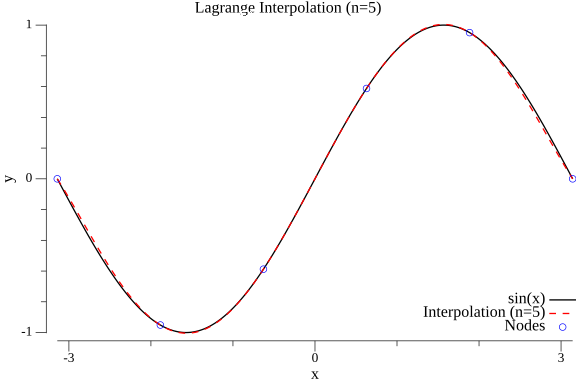
\includegraphics[width=1.0\linewidth]{material/sin/interp/sin_interp_n05.png}
  \end{minipage}
  \hfill
  \begin{minipage}[b]{0.48\linewidth}
    \centering
    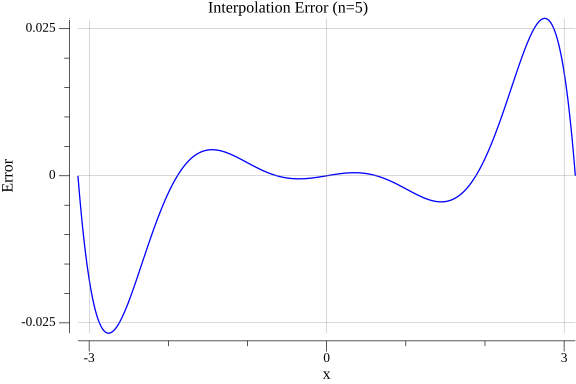
\includegraphics[width=1.0\linewidth]{material/sin/interp/sin_interp_err_n05.png}
  \end{minipage}
\end{figure}

\begin{figure}[H]
  \centering
  \caption{$f(x) = \sin(x)$の等間隔補間（$n=11$次多項式）}
  \label{fig:sin-interp-last}
  \vspace{5pt}
  \begin{minipage}[b]{0.48\linewidth}
    \centering
    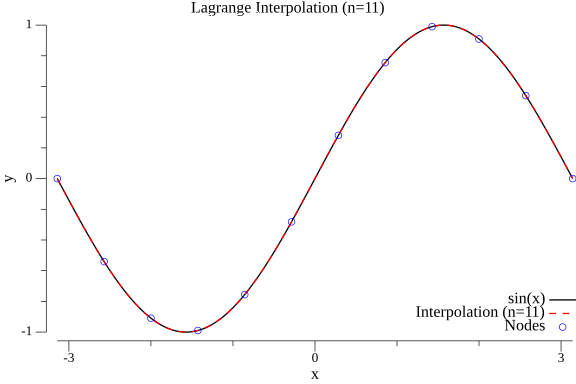
\includegraphics[width=1.0\linewidth]{material/sin/interp/sin_interp_n11.png}
  \end{minipage}
  \hfill
  \begin{minipage}[b]{0.48\linewidth}
    \centering
    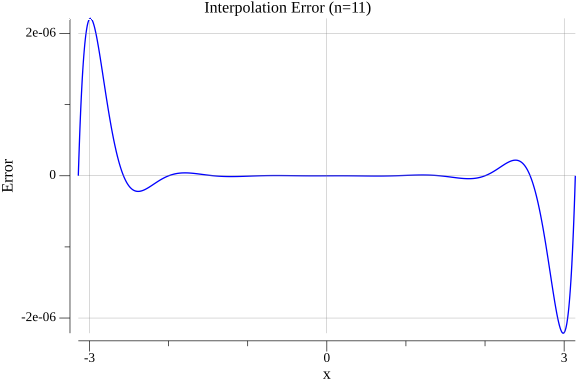
\includegraphics[width=1.0\linewidth]{material/sin/interp/sin_interp_err_n11.png}
  \end{minipage}
\end{figure}


\label{subsec:runge_phenomenon}
  
    このような関数に対しては等間隔点でも良好な近似が得られることが分かる．

  \subsection{ルンゲ現象：等間隔点による補間が失敗する例}
    しかし，すべての関数に対して等間隔点による補間が成功するわけではない．
    代表的な反例として，次の関数を考える．
    \[f(x) = \frac{1}{1 + 25x^2}.\]
    
    この関数は一見すると単純であるが，この式の等間隔標本点の補間多項式は区間の端点付近で急激に変化する特性を持つ．
    この関数に対して等間隔点による補間を行うと，次のように予想外の振動が生じる．
  
    \clearpage  
    % =========================================================
    % Goプログラム (runge_unified.go) が生成した
    % 等間隔補間の可視化ファイルを読み込む
    % =========================================================
    % ルンゲ関数の等間隔補間による比較図

\begin{figure}[H]
  \centering
  \caption{$f(x) = \frac{1}{1+25x^2}$の等間隔補間（$n=4$次多項式）}
  \label{fig:runge-equidistant-first}
  \vspace{5pt}
  \begin{minipage}[b]{0.48\linewidth}
    \centering
    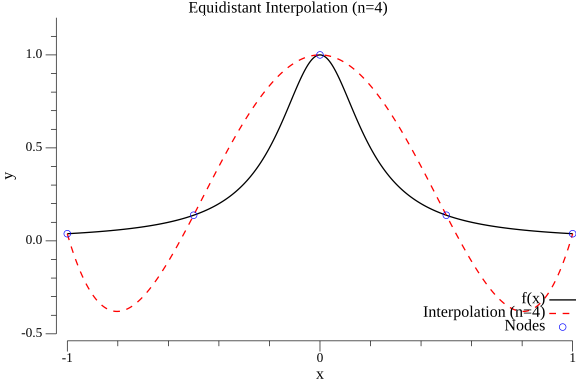
\includegraphics[width=1.0\linewidth]{material/runge/equidistant/runge_n04.png}
  \end{minipage}
  \hfill
  \begin{minipage}[b]{0.48\linewidth}
    \centering
    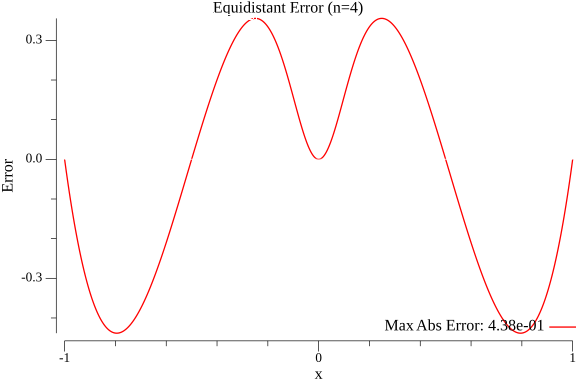
\includegraphics[width=1.0\linewidth]{material/runge/equidistant/runge_err_n04.png}
  \end{minipage}
\end{figure}

\begin{figure}[H]
  \centering
  \caption{$f(x) = \frac{1}{1+25x^2}$の等間隔補間（$n=7$次多項式）}
  \label{fig:runge-equidistant-2}
  \vspace{5pt}
  \begin{minipage}[b]{0.48\linewidth}
    \centering
    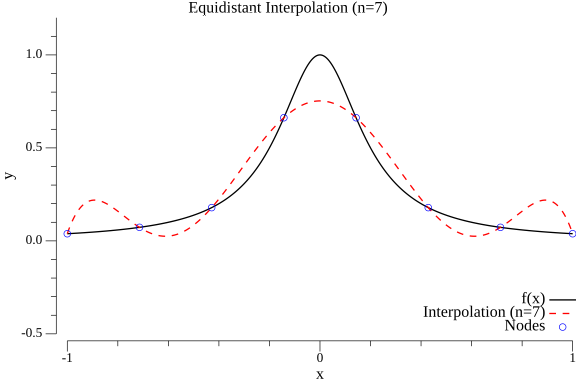
\includegraphics[width=1.0\linewidth]{material/runge/equidistant/runge_n07.png}
  \end{minipage}
  \hfill
  \begin{minipage}[b]{0.48\linewidth}
    \centering
    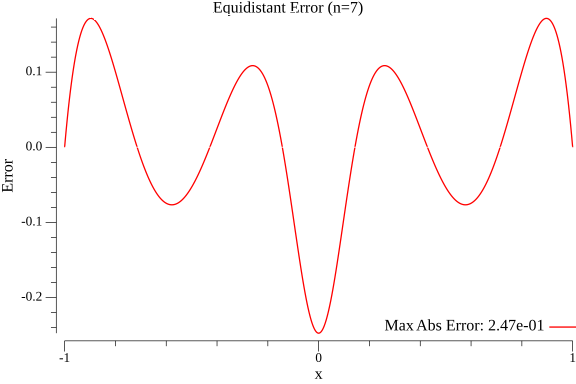
\includegraphics[width=1.0\linewidth]{material/runge/equidistant/runge_err_n07.png}
  \end{minipage}
\end{figure}

\begin{figure}[H]
  \centering
  \caption{$f(x) = \frac{1}{1+25x^2}$の等間隔補間（$n=15$次多項式）}
  \label{fig:runge-equidistant-last}
  \vspace{5pt}
  \begin{minipage}[b]{0.48\linewidth}
    \centering
    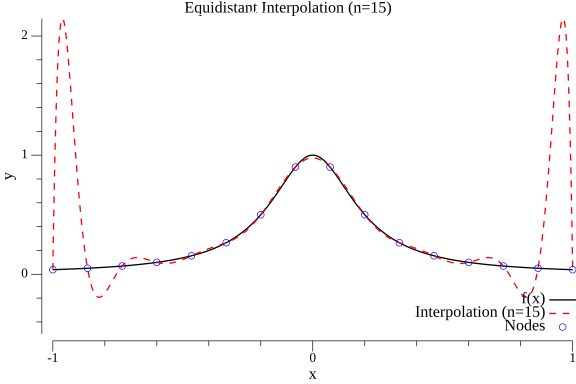
\includegraphics[width=1.0\linewidth]{material/runge/equidistant/runge_n15.png}
  \end{minipage}
  \hfill
  \begin{minipage}[b]{0.48\linewidth}
    \centering
    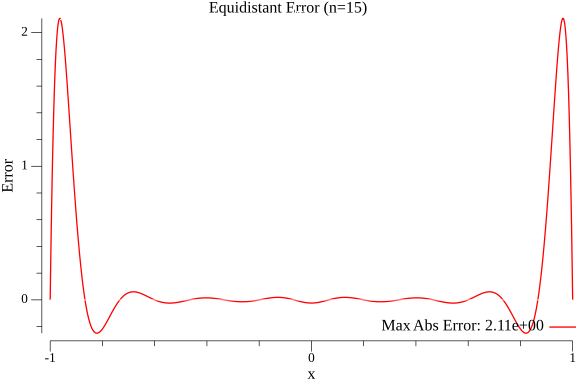
\includegraphics[width=1.0\linewidth]{material/runge/equidistant/runge_err_n15.png}
  \end{minipage}
\end{figure}



  \label{subsec:chebyshev_solution}
    このような現象を\textbf{ルンゲ現象}という．
    多項式の次数を増やしても誤差が減少するどころか，むしろ悪化してしまう場合がある．

  \subsection{チェビシェフ多項式を用いた標本点による補間：失敗例の改善}
    ルンゲ現象を回避するための一つの方法として，振幅が大きくなった端点付近に標本点を集中させる方法がある．
    その手法の一つとして，次のようなチェビシェフ多項式 $T_{n+1}(x)$ の零点を標本点として用いる方法が知られている．
    \begin{equation}
      x_k = \cos \left( \frac{2k + 1}{2(n + 1)} \pi \right) \quad (k = 0, 1, \dots, n).
    \end{equation}
    
    チェビシェフ多項式の零点を用いると，標本点が区間の両端に集中するため，補間多項式の振動が抑制される．
    同じルンゲ関数に対してチェビシェフ多項式の零点を用いた結果は以下の通りである．
    \clearpage
    % =========================================================
    % Goプログラム (runge_unified.go) が生成した
    % チェビシェフ補間の可視化ファイルを読み込む
    % =========================================================
    \input{material/runge/runge_chebyshev_result}

    チェビシェフ多項式の零点を用いた結果（図 \ref{fig:runge-chebyshev-first}～図 \ref{fig:runge-chebyshev-last}）は
    等間隔標本点を採用した結果（図 \ref{fig:runge-equidistant-first}～図 \ref{fig:runge-equidistant-last}）に比べて，振動を大幅に抑制できている．
    ただし，この多項式は標本点を通るだけであり，区間全体における誤差が最も小さい点であるかといわれるとそうではない．
    
    このように，補間多項式の標本点の選択は，補間する関数の性質に大きく依存する重要な要素である．
    次章では最も良い近似を得るためのゴールの一つとして最良近似多項式と呼ばれるものについて述べる．
    最良近似多項式を大まかに説明すると，区間全体における誤差を最小化する多項式である．
\clearpage